\documentclass{article}
\usepackage[margin=1in]{geometry}
\usepackage{graphicx}
\usepackage{amsmath}
\usepackage{array}
\usepackage{float}

\title{CSCI/ROBO 7000/4830: Deep Reinforcement Learning and Robotics \ Fall 2025 \ Homework \#1: The Wormhole Grid}
\author{Steve Gillet}
\begin{document}
\maketitle
\section*{Part 1: Policy and Value Analysis [40 Points]}

\subsection*{1. Policy Evaluation [15/40 Points]}

Consider the following simple, "go-up-and-right" policy, $\pi_{simple}$: in every state, the agent attempts to move North. If North is blocked, it tries to move East. If both are blocked, it moves South.

\subsubsection*{A) Calculate the state-value function, $V^{\pi_{simple}}(s)$, for this policy for all states. Fill in your values on a 4x4 grid.}

The state-value function is calculated using the Bellman expectation equation:

\begin{figure}[H]
    \centering
    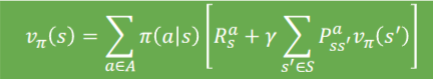
\includegraphics[width=0.4\textwidth]{bellmanExpectation.png}
\end{figure}

Since the environment is deterministic and the policy selects a single action per state, this simplifies to:

\[
v^\pi(s) = r + \gamma v^\pi(s')
\]

where $s'$ is the next state and $r$ is the reward (with $\gamma = 0.9$).

The values are as follows (grid with row 0 at the top):

\begin{center}
\begin{tabular}{|c|c|c|c|}
\hline
38.6 & 44 & 50 & 0 \\
\hline
33.74 & N/A & -46 & 0 \\
\hline
29.366 & -39.16 & -42.4 & -50 \\
\hline
25.4294 & -36.244 & -39.16 & -46 \\
\hline
\end{tabular}
\end{center}

\subsubsection*{B) Show the setup for your calculations for at least two non-terminal states.}

There's this recursive nature to the Bellman expectation equation in this form where in order to get the value of the current state you need to know the reward for the transition plus the value of the next state.
In order to know the value of the next state you have to know the value of the one after that all the way back to the terminal states.
So the (0,0) state depends on (0,1) which depends on (0,2) which is 50 because (0,3) is the terminal state which has a value of 0 but transitioning into it gives a reward of 50.

For state (0,0):

\[
v(0,0) = -1 + \gamma \left( -1 + \gamma \cdot 50 \right)
\]

For state (3,1):

\[
v(3,1) = -1 + \gamma \left( -1 + \gamma \left( -1 + \gamma \left( -1 + \gamma \cdot (-50) \right) \right) \right)
\]

\subsubsection*{2. Optimal Value and Policy [15/40 Points]}

To compute the optimal values using Value Iteration, we iteratively update the value function according to the Bellman optimality equation:

\begin{equation}
v_{k+1}(s) = \max_a \left[ r(s, a, s') + \gamma v_k(s') \right]
\end{equation}

for all non-terminal states $s$, initializing $v_0(s) = 0$. Terminal states (G, T) have value 0, and obstacle (O) and wormhole entry (W) are marked N/A as they are not occupiable. Here are the value grids after the first few iterations (rounded to 2 decimal places for display):

\begin{figure}[H]
    \centering
    \begin{minipage}{0.3\textwidth}
        \centering
        \begin{tabular}{|c|c|c|c|}
        \hline
        0.00 & 0.00 & 0.00 & 0.00 \\
        \hline
        0.00 & N/A & N/A & 0.00 \\
        \hline
        0.00 & 0.00 & 0.00 & 0.00 \\
        \hline
        0.00 & 0.00 & 0.00 & 0.00 \\
        \hline
        \end{tabular}
        \vspace{0.5em}
        \small $V_0$
    \end{minipage}
    \hfill
    \begin{minipage}{0.3\textwidth}
        \centering
        \begin{tabular}{|c|c|c|c|}
        \hline
        -1.00 & -1.00 & 50.00 & 0.00 \\
        \hline
        -1.00 & N/A & N/A & 0.00 \\
        \hline
        -1.00 & -1.00 & -1.00 & -1.00 \\
        \hline
        -1.00 & -1.00 & -1.00 & -1.00 \\
        \hline
        \end{tabular}
        \vspace{0.5em}
        \small $V_1$
    \end{minipage}
    \end{figure}

\begin{figure}[H]
    \centering
    \begin{minipage}{0.3\textwidth}
        \centering
        \begin{tabular}{|c|c|c|c|}
        \hline
        -1.90 & 44.00 & 50.00 & 0.00 \\
        \hline
        -1.90 & N/A & N/A & 0.00 \\
        \hline
        -1.90 & -1.90 & -1.90 & -1.90 \\
        \hline
        -1.90 & -1.90 & -1.90 & -1.90 \\
        \hline
        \end{tabular}
        \vspace{0.5em}
        \small $V_2$
    \end{minipage}
    \hfill
    \begin{minipage}{0.3\textwidth}
        \centering
        \begin{tabular}{|c|c|c|c|}
        \hline
        38.60 & 44.00 & 50.00 & 0.00 \\
        \hline
        33.74 & N/A & N/A & 0.00 \\
        \hline
        29.37 & 25.43 & 21.89 & 18.70 \\
        \hline
        25.43 & 21.89 & 18.70 & 15.83 \\
        \hline
        \end{tabular}
        \vspace{0.5em}
        \small $V^*$
    \end{minipage}
\end{figure}

The process continues until convergence (changes < $10^{-6}$). The converged optimal values $V^*(s)$ are as shown above. The optimal policy $\pi^*(a|s)$ (arrows indicating one best action per state; in cases of ties, one is shown):

\begin{center}
\begin{tabular}{|c|c|c|c|}
\hline
$\rightarrow$ & $\rightarrow$ & $\rightarrow$ & $G$ \\
\hline
$\uparrow$ & $O$ & $W$ & $T$ \\
\hline
$\uparrow$ & $\leftarrow$ & $\leftarrow$ & $\leftarrow$ \\
\hline
$\uparrow$ & $\uparrow$ & $\uparrow$ & $\uparrow$ \\
\hline
\end{tabular}
\end{center}

\end{document}